\documentclass{article}
\usepackage[slovak]{babel}
\usepackage[utf8]{inputenc}

\usepackage{indentfirst}
\usepackage{graphicx}

\begin{document}
    \begin{titlepage}
        \begin{center}
            \textsc{\Huge Vysoké učení technické v~Brně\\
            		\huge Fakulta informačních technologií\\}
            \vspace{\stretch{0.382}}
            {\LARGE ISA - Síťové aplikace a~správa sítí\\}\vspace{2em}
            {\Large dokumentácia k 2.variante projektu\\}\vspace{2em}
            \Huge dns-export\\
            \vspace{\stretch{0.618}}
        \end{center}
        {\Large \today \hfill Tomáš Nereča}\vspace{-2em}
    \end{titlepage}

    \tableofcontents
        \thispagestyle{empty}
        \newpage
        \setcounter{page}{1}
    \newpage
    
    \section{Úvod}

        \textbf{dns-export} je aplikácia na spracovávanie dát protokolu \emph{DNS (Domain Name System)}.
        Aplikácia teda musí vedieť identifikovať a spracovať \emph{paket} daného protokolu.
        Jednotlivé pakety môže buď čerpať z \emph{pcap} súboru alebo odchytávať v reálnom čase
        zo sieťového rozhrania.

        Zo spracovaných dát vytvára štatistiky, ktoré v časovom intervale posiela protokolom \emph{Syslog}
        na centrálny logovací server alebo jednoducho vypisuje na štandardný výstup. Zbierané štatistiky sú
        \texttt{domain-name rr-type rr-answer count}.
    
    \section{Návrh aplikácie}

        \subsection{Objektový návrh}
        Svoju aplikáciu som sa rozhodol naprogramovať objektovo. Dodržiaval som štruktúru jedna \emph{trieda}
        na jeden zdrojový súbor. Každá trieda má svoju významom vyhradenú funkciu. 

        \subsection{Spracovanie paketov}
        Aplikácia spracuje vstupné argumenty a po ich validácii sa buď spustí spracovanie pcap súboru, alebo odchytávanie
        paketov zo sieťového rozhrania. Pre každý spracovávaný paket sa vytvorí objekt držiaci dáta paketu.

        V tomto objekte sa najprv spracujú jednotlivé hlavičky paketu. Ak sa zistí, že paket obsahuje odpovede na DNS otázky,
        Vytvorí sa pre každú odpoveď objekt, ktorý tieto odpovede spracováva.

        \subsection{Ukladanie štatistík}
        Po úspešnom spracovaní odpovedí sa každá odpoveď pridá do objektu, ktorý obsahuje kolekciu všetkých nazbieraných štatistík.
        Pomocou metódy sa zistí, či sa daná štatistická informácia v objekte už nachádza a v tom prípade sa len inkrementuje počítadlo.
        
        \subsection{Odosielanie a výpis štatistík}
        Po prečítaní z pcap súboru sa štatistiky uložené v objekte odošlú na server ak je zadaný alebo vypíšu na štandardný výstup.
        V prípade živého odchytávania sa pred jeho spustením vytvorí separátne vlákno, ktoré bude v zadanom časovom intervale
        odosielať všetky doposiaľ nazbierané štatistiky. Okrem toho bude aplikácia pri odchytení signálu \textbf{SIGUSR1} volať funkciu
        na výpis štatistík na štandardný výstup.
        
    \section{implementácia}
    
        \subsection{DnsExport.cpp}
        Po spustení aplikácie je vytvorený objekt tejto triedy a zavolaná funkcia \textbf{Main()}. Nastaví sa odchýtavanie signálov
        a na základne vstupných argumentov načítaných pomocou vstavanej funkcie \textsc{getopt()}\footnote{http://man7.org/linux/man-pages/man3/getopt.3.html} sa rozhodne, či sa spustí funkcia
        \textbf{sniffInterface()} alebo \textbf{sniffFile()}. 
        
        V prvom prípade sa pred započatím odchytávania spustí funkcia \textbf{sendingLoop()},
        ktorá sa v separátnom vlákne stará o pravidelné odosielanie na Syslog server. Pre odoslanie volá funkcia \textbf{sendStats()}, ktorá si volá
        pomocné funkcie na vytvorenie správ ako napr.: \textbf{getMessages()} alebo \textbf{getFormattedTime()} a následne \emph{UDP} protokolom 
        odosiela správy. Správa nie je dlhšia ako 1 kB a jednotlivé štatistiky sú oddelené znakom '|'.

        V druhom prípade ak nebol zadaný Syslog server, je po prečítaní súboru zavolaná funkcia \textbf{getMessages()}, ktorá štatistiky vypíše
        na štandardný výstup a aplikácia končí. Rovnaká funkcia je volaná aj pri prijatí signálu \textbf{SIGUSR1}.

        O všetky akcie ohľadom odchytávania paketov sa stará knižnica \textbf{libpcap}\footnote{https://www.tcpdump.org/pcap.html}. Pre každý paket
        je volaná \emph{callback} funkcia \textbf{pcapHandler()}. Tam je vytvorený objekt triedy \textbf{DnsPacket} a zavolaná funkcia \textbf{Parse()}.

        Ak boli v pakete nájdené validné DNS odpovede - \emph{answers}, je zavolaná funkcia \textbf{addRecords()}, ktorá do globálnej premennej \textbf{recordList} pridá nový
        objekt triedy \textbf{DnsRecord}, ak sa daná štatistika v liste ešte nenachádza, alebo len zvýši počítadlo u nájdenej štatistiky.

        \subsection{DnsPacket.cpp}
        Vo funkcii \textbf{Parse()} je najprv zavolaná funkcia \textbf{getTransProt()}. Tá parsuje \emph{ethernet} hlavičku (podporované typy sú IPv4 a IPv6)
        a následne zistí transportný protokol (podporované typy sú UDP a TCP) a skočí na pozíciu, kde by sa mala nachádzať DNS hlavička.

        Parsovanie DNS hlavičky začína vo funkcii \textbf{dnsParse()}. Tam prebehnú validácie, či ide skutočne o DNS paket. \emph{query} pakety sú
        ignorované, aplikácia pracuje len s answers. Ak sú nájdené answers, je zavolaná funkcia \textbf{parseRRSet()}, kde je hneď na začiatku zavolaná funkcia \textbf{skipQuestion()}, ktorá
        skočí na pozíciu prvej answer.

        Pre každú answer je vytvorený objekt triedy \textbf{DnsRR}, ktorý spracuje dáta a nastaví pozíciu na ďalšiu answer. Ak boli získané nejaké dáta, objekt je uložený do listu
        \textbf{Answers}.

        \subsection{DnsRR.cpp}
        Každá answer začína \emph{domain-name}, ktorý je získaný funkciou \textbf{readDomainName()}. Ak sa podarí získať domain-name, nasleduje získanie typu záznamu - \emph{rr-type} a dĺžky dát.
        Vo funkcii \textbf{applyParser()} je \textbf{switch}, v ktorom sa na základe typu záznamu rozhodne ktorý z parserov\footnote{Konkrétnejší popis jednotlivých parserov je v komentároch v zdrojovom kóde.} pre dáta použiť. Okrem toho sa typ uloží ako \emph{string}
        hodnota pre jednoduchšie ukladanie štatistík. Ak sa podarilo získať dáta, je vrátená pozícia za odpoveďou a aplikácia pokračuje parsovaním ďalšej answer.

        \subsection{Helpers.cpp}
        Táto trieda obsahuje makrá pre logovanie \textbf{LOGGING} a ukončovanie aplikácie ak nastane problém \textbf{ERR_RET} pomocné statické funkcie.

        Funkcia \textbf{ToHex()} prevedie netlačiteľný znak do hexadecimálneho tvaru, napr.: \texttt{0x01}. Je používaná ak sa napríklad v domain-name alebo \texttt{TXT}
        zázname objaví netlačiteľný znak.

        Funkcia \textbf{Base64Encode()} je využívaná parseroch pre záznamy typu \texttt{DNSKEY, DS a RRSIG}. Kóduje bajtové pole ako base64 string, ktorý sa zobrazí v štatistikách.
        Funkcia je dostupná na githube\footnote{https://github.com/ReneNyffenegger/cpp-base64/blob/master/base64.cpp} pod \emph{Zlib} licenciou. 
    
    \section{Zaujímavé časti kódu}
        \subsection{LINUX_SLL datalink}
        Pri odchytávaní na všetkých rozhraniach ("any"), nemajú pakety ethernet hlavičku ale tzv. \emph{"linux-coocked header"}.
        To sa dá zistiť pomocou funkcie \textbf{pcap_datalink()}. Ak ide \texttt{LINUX_SLL_DATALINK}, hlavička je parsovaná iným spôsobom ako ethernet:
        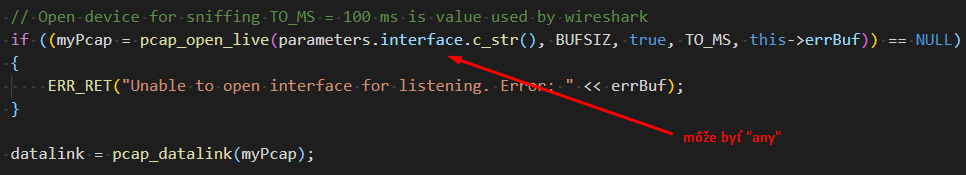
\includegraphics {datalink.png}
        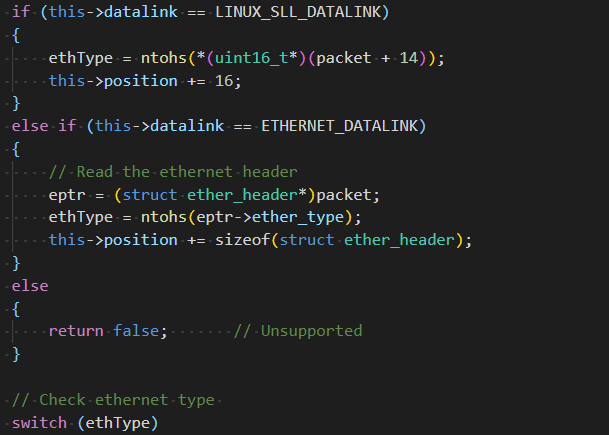
\includegraphics {ethernet.png}

        \subsection{Odosielanie na Syslog}
        Pri spustení vlákna na odosielanie sa najprv vyčká 20 ms a až potom sa spustí cyklus na odosielanie. Pretože aplikácia využíva parameter \textbf{to_ms}
        vo funkcii \textbf{pcap_open_live()}, chceme aby sa stihli vytvoriť všetky štatistiky pred odoslaním. Kód je inšpirovaný vláknom na stránke
        cplusplus.com\footnote{http://www.cplusplus.com/forum/beginner/91449/}
        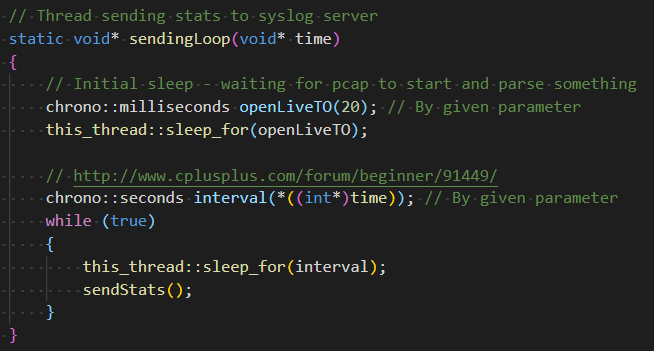
\includegraphics {loop.png}

        \subsection{Pole "hostname" v Syslog správe}
        RFC 5424\footnote{https://tools.ietf.org/html/rfc5424} špecifikuje prioritu. Aplikácia nepredpokladá existenciu FQDN ani statickú IP adresu, preto
        sa najprv pokúsi získať hostname a až v prípade neúspechu ip adresu.
        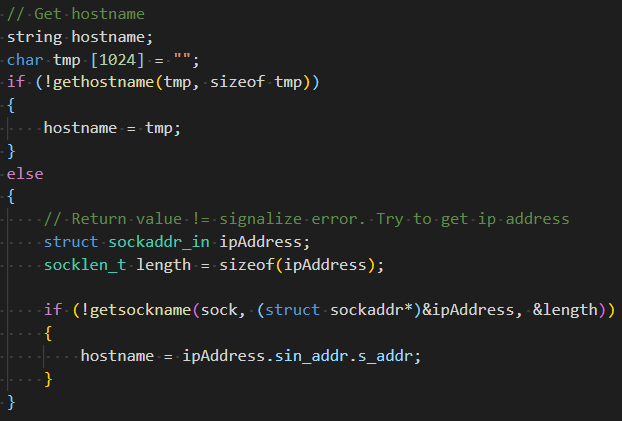
\includegraphics {hostname.png}

        \subsection{Získanie aktuálneho timestampu}
        Syslog správa potrebuje timestamp v špecifickom tvare. Kód je inšpirovaný vláknom na stránke
        codereview.stackexchange.com\footnote{https://codereview.stackexchange.com/questions/11921/getting-current-time-with-milliseconds}
        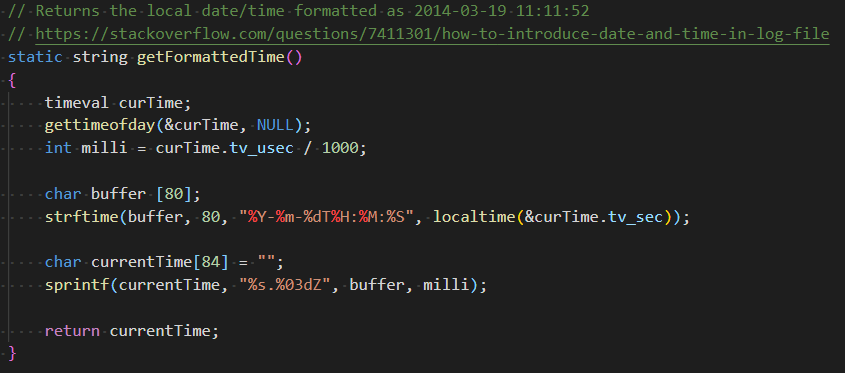
\includegraphics {timestamp.png}


        \subsection{Vytvorenie správ na odoslanie}
        Aplikácia vytvára správy s dĺžkou nepresahujúcou 1KB. Na Syslog server je v jednej správe posielaných viac štatistík oddelených znakom \texttt{|}.
        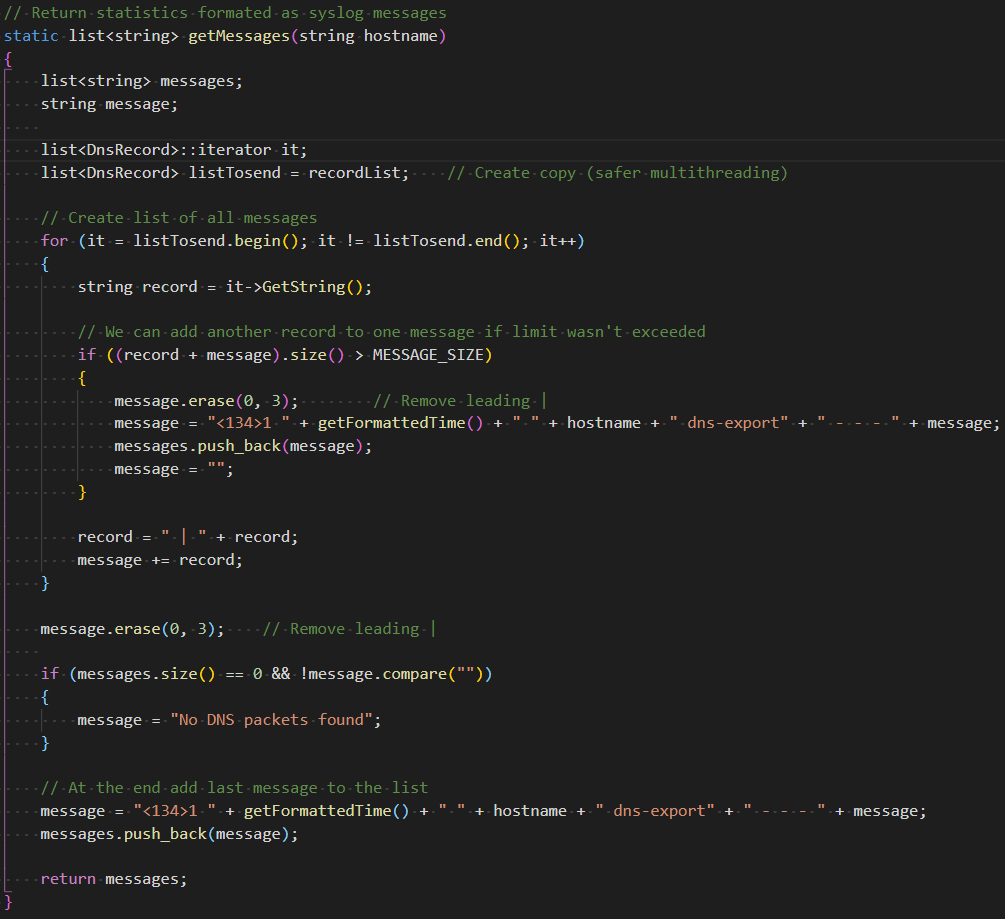
\includegraphics {messages.png}

    \section{Použitie}
        \subsection{Čítanie pcap súboru}
        Aplikácia sa spúšťa s argumentmi \textbf{-r} a \textbf{-s}:\\
        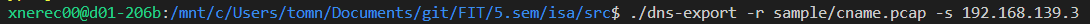
\includegraphics {r1.png}
        V tomto prípade sa na \textbf{stdout} nič nevypíše, štatistiky sú odoslané na Syslog server, napr.:\\
        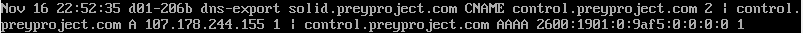
\includegraphics {r2.png}
        V prípade, že nie je zadaný Syslog server sa štatistiky vypíšu na \textbf{stdout}:\\
        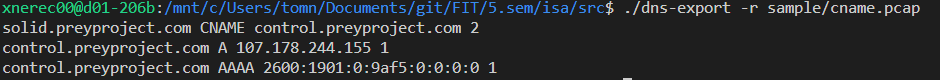
\includegraphics {r3.png}

        \subsection{Odchytávanie na rozhraní}
        Aplikácia sa spúšťa s argumentmi \textbf{-i}, \textbf{-s} a \textbf{-t}:\\
        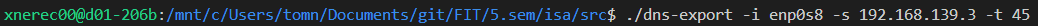
\includegraphics {i1.png}
        V tomto prípade budú štatistiky odosielané na Syslog server každých 45 sekúnd. Ak nie je zadaný argument \textbf{-t},
        štatistiky sú odosielané každých 60 sekúnd. Ak nie je zadaný argument \textbf{-s}, štatistiky sa neodosielajú.

        \subsection{Zaslanie signálu SIGUSR1}
        Pri odchytávaní na rozhraní sa štatistiky vypíšu na \textbf{stdout} pri zaslaní signálu \texttt{SIGUSR1}:\\
        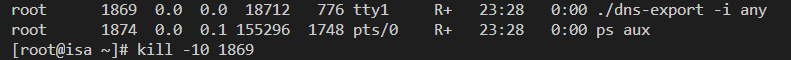
\includegraphics {i2.png}
        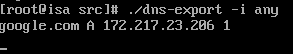
\includegraphics {i3.png}
    
    \newpage
    \section{Prílohy}
        \subsection{Diagram konečného automatu}
            \newpage
            
        \subsection{LL gramatika}
            \begin{enumerate}
                % NESAHAT - zhenodnotí čísla v tabulce LL gramatiky!
                \item \texttt{<program> -> declare function <functionDecl> eol <program>}
                \item \texttt{<program> -> function <functionDef> eol <program>}
                \item \texttt{<program> -> scope <statementList> end scope}
                
                \item \texttt{<functionDecl> -> <functionHeader>}
                \item \texttt{<functionDef> -> <functionHeader> eol <statementList> end function}
                
                \item \texttt{<functionHeader> -> identifier ( <functionParams> ) as type}
                
                \item \texttt{<functionParams> -> <functionParam> <nextFuncParam>}
                \item \texttt{<functionParams> -> epsilon}
                
                \item \texttt{<nextFuncParam> -> , <functionParam> <nextFuncParam>}
                \item \texttt{<nextFuncParam> -> epsilon}
                
                \item \texttt{<functionParam> -> identifier as type}
                
                \item \texttt{<statementList> -> <statement> eol <statementList>}
                \item \texttt{<statementList> -> epsilon}
                
                \item \texttt{<statement> -> dim <declaration>}
                \item \texttt{<statement> -> identifier = <expression>}
                \item \texttt{<statement> -> input identifier}
                \item \texttt{<statement> -> print <printArgs>}
                \item \texttt{<statement> -> if <expression> then eol <statementList> <else>}
                \item \texttt{<statement> -> do while <expression> eol <statementList> loop}
                \item \texttt{<statement> -> return identifier}
                
                \item \texttt{<declaration> -> identifier as type}
                \item \texttt{<declaration> -> identifier as type = <expression>}
                
                \item \texttt{<printArgs> -> <expression> ;}
                \item \texttt{<printArgs> -> <expression> ; <printArgs>}
                
                \item \texttt{<else> -> elseif <expression> then eol <else> end if}
                \item \texttt{<else> -> else eol <statementList> end if}
                \item \texttt{<else> -> end if}
                
                \item \texttt{<expression> ->} vyhodnocuje se precedenční syntaktickou analýzou
            \end{enumerate}
        \newpage
        
        \subsection{LL tabuľka}
        \newcommand{\tterm}[1]{\rotatebox[origin=c]{90}{\texttt{#1}}}
            \begin{tabular}{|r|*{10}{c|}}
                \hline
                & \tterm{declare} & \tterm{function} & \tterm{scope} & \tterm{identifier} & \tterm{dim} &
                \tterm{input} & \tterm{print} & \tterm{if} & \tterm{do} & \tterm{return} \\\hline \hline
                \texttt{<program>} & 1 & 2 & 3 &&&&&&& \\\hline
                \texttt{<functionDecl>} &&&& 4 &&&&&& \\\hline
                \texttt{<functionDef>} &&&& 5 &&&&&& \\\hline
                \texttt{<functionHeader>} &&&& 6 &&&&&& \\\hline
                \texttt{<functionParams>} &&&& 7, 8 &&&&&& \\\hline
                \texttt{<nextFuncParam>} &&&&&&&&&& \\\hline
                \texttt{<functionParam>} &&&& 11 &&&&&& \\\hline
                \texttt{<statementList>} &&&& 12 & 12 & 12 & 12 & 12 & 12 & 12 \\\hline
                \texttt{<statement>} &&&& 15 & 14 & 16 & 17 & 18 & 19 & 20 \\\hline
                \texttt{<declaration>} &&&& 21, 22&&&&&& \\\hline
                \texttt{<else>} &&&& 23, 24&&&&&& \\\hline
            \end{tabular}
            
            \begin{tabular}{|r|*{9}{c|}}
                \hline
                & \tterm{elseif} & \tterm{else} & \tterm{end} & \tterm{loop} & \tterm{eol} &
                \tterm{(} & \tterm{)} & \tterm{=} & \tterm{,} \\\hline \hline
                \texttt{<program>} &&&&&&&&& \\\hline
                \texttt{<functionDecl>} &&&&&&&&& \\\hline
                \texttt{<functionDef>} &&&&&&&&& \\\hline
                \texttt{<functionHeader>} &&&&&&&&& \\\hline
                \texttt{<functionParams>} &&&&&&& 8 && \\\hline
                \texttt{<nextFuncParam>} &&&&&&& 10 && 9 \\\hline
                \texttt{<statementList>} & 13 & 13 & 13 & 13 &&&&& \\\hline
                \texttt{<statement>} &&&&&&&&& \\\hline
                \texttt{<declaration>} &&&&&& 23, 24&&& \\\hline
                \texttt{<else>} & 25 & 26 & 27 &&&&&& \\\hline
            \end{tabular}
        \newpage

        \subsection{Precedenčná tabuľka}

        \begin{center}
        \begin{tabular}{|c||c|c|c|c|c|c|c|c|c|c|c|c|c|c|c|c|c|c|}
        \hline
                    &  =  & $<>$ & $<$= & $>$= & $<$ & $>$ &  +  &  -  &  *   &  /  & \textbackslash &  (  &  )  & \$  \\ 
        \hline
        \hline  
           =        & $>$ &  $>$ &  $>$ &  $>$ & $>$ & $>$ & $<$ & $<$ &  $<$ & $<$ & $<$            & $<$ & $>$ & $>$ \\ 
        \hline  
          $<>$      & $>$ &  $>$ &  $>$ &  $>$ & $>$ & $>$ & $<$ & $<$ &  $<$ & $<$ & $<$            & $<$ & $>$ & $>$ \\
        \hline  
          $<$=      & $>$ &  $>$ &  $>$ &  $>$ & $>$ & $>$ & $<$ & $<$ &  $<$ & $<$ & $<$            & $<$ & $>$ & $>$ \\
        \hline  
          $>$=      & $>$ &  $>$ &  $>$ &  $>$ & $>$ & $>$ & $<$ & $<$ &  $<$ & $<$ & $<$            & $<$ & $>$ & $>$ \\
        \hline  
          $<$       & $>$ &  $>$ &  $>$ &  $>$ & $>$ & $>$ & $<$ & $<$ &  $<$ & $<$ & $<$            & $<$ & $>$ & $>$ \\
        \hline        
          $>$       & $>$ &  $>$ &  $>$ &  $>$ & $>$ & $>$ & $<$ & $<$ &  $<$ & $<$ & $<$            & $<$ & $>$ & $>$ \\
        \hline  
           +        & $>$ &  $>$ &  $>$ &  $>$ & $>$ & $>$ & $>$ & $>$ &  $<$ & $<$ & $<$            & $<$ & $>$ & $>$ \\
        \hline  
           -        & $>$ &  $>$ &  $>$ &  $>$ & $>$ & $>$ & $>$ & $>$ &  $<$ & $<$ & $<$            & $<$ & $>$ & $>$ \\ 
        \hline  
          */        & $>$ &  $>$ &  $>$ &  $>$ & $>$ & $>$ & $>$ & $>$ &  $>$ & $>$ & $>$            & $<$ & $>$ & $>$ \\ 
        \hline  
\textbackslash      & $>$ &  $>$ &  $>$ &  $>$ & $>$ & $>$ & $>$ & $>$ &  $<$ & $<$ & $>$            & $<$ & $>$ & $>$ \\
        \hline  
           (        & $<$ &  $<$ &  $<$ &  $<$ & $<$ & $<$ & $<$ & $<$ &  $<$ & $<$ & $<$            & $<$ &  =  &     \\  
        \hline  
           (        & $>$ &  $>$ &  $>$ &  $>$ & $>$ & $>$ & $>$ & $>$ &  $>$ & $>$ & $>$            &     & $>$ & $>$ \\ 
        \hline  
          \$        & $<$ &  $<$ &  $<$ &  $<$ & $<$ & $<$ & $<$ & $<$ &  $<$ & $<$ &  $<$            & $<$ &     &     \\ 
        \hline  
        \end{tabular}
    \end{center}
\end{document}